\subsection{Long-Slit Spectroscopy in L/M- and N-bands}\label{lss:overview}
\subsubsection{The workflow cascades}\label{lss:cascade_overview}
The purpose of the pipeline is to correct or remove contributions from
the instrument, telescope, and atmosphere and generate science-grade
data products for the L/M- and N-band \ac{LSS}
mode. Since the detector properties are not fully specified, especially of the new Geosnap, we currently assume
basically the same reduction cascade for both spectral ranges LM and
N, respectively. The only major difference at the time being is the absence of \ac{WCU} laser sources in the N-band, which are only available during \ac{AIT} phase to generate a first guess of the pixel-to-wavelength relation. Therefore the first guess wavelength solution in the N-band will be based on that \ac{AIT} data. As we assume the instrument to be very stable, that approach should be sufficient for the low-resolution N-band spectroscopy. In the LM range, two fix-frequency lasers ($@3.39$µm and $@5.26$µm) and one tuneable ($4.68....4.78$µm) is foreseen in the \ac{WCU} to be taken on daily basis (cf. \cite{METIS-calibration_plan}). Although mainly foreseen to be used for the high-resolution spectroscopy \ac{LMS} mode, we can use these laser sources for the LM-band \ac{LSS} as well.

Special emphasis has to be drawn to the effects of the Earth's
atmosphere in several respects:
\begin{itemize}
\item Wavelength calibration: Absorption/emission features are intended to be
  used for the wavelength calibration. Thus, a good knowledge on /
  identification of these features is crucial for the accuracy of the
  wavelength calibration.
\item Telluric correction: In the MIR regime telluric absorption is
  one of the most dominant effects visible in spectra. Modelling
  approaches like \texttt{molecfit} heavily rely on accurate
  atmospheric input profiles, which represent the actual state and
  composition of the Earth's atmosphere. This especially applies to
  the \ac{PWV} content since this is the most
  dominant and most variable species.
\item Atmospheric dispersion: \ac{METIS} will have \ac{ADC}s compensating the
  effect of atmospheric dispersion. However, for technical reasons
  these ADCs are fixed at several positions. This means that the
  compensation is only partially. This leads to two practical effects:
  (a) wavelength-dependent slit losses, and (b) distortions in both,
  the spatial and the spectral direction (see \cite{METIS-ADC_study}
  for more details). For both, the pipeline needs to correct
  for. It is foreseen to determine these slitlosses on yearly basis with a separate calibration task (cf. \cite{METIS-calibration_plan}) and create a slit-loss table to be included in the static calibration database.
\end{itemize}

%However, to keep flexibility and independence of both branches, we
%define different recipes for the time being, although they will be
%mostly based on the same algorithms. We therefore focus here on the LM-band only.

Figure~\ref{Fig:LMLssAssomap} shows the reduction cascade and the association map for the recipes handling L/M-long-slit
spectroscopy data.  Table~\ref{Tab:LMLssDatProc} contains the data processing table for this mode. For the N-band \ac{LSS} mode the cascade and the data processing table is given in Fig.\ref{Fig:NLssAssomap} and Table~\ref{Tab:NLssDatProc}, respectively (cf. also Fig.~\ref{Fig:LSScascadelegend}).

In general, there are four major steps in each of the two cascades:
\begin{itemize}
    \item \textbf{Preparation step:} This contains the recipes, which are invoked only rarely, e.g. after major instrument interventions, or on monthly/yearly basis to update the static calibration database. These recipes are therefore not shown in the cascade in Figs.~\ref{Fig:LMLssAssomap} and \ref{Fig:NLssAssomap} and the corresponding data processing tables. In case of the \ac{LSS} pipeline this concerns the creation of the gain maps/linearity checks (see Section~\ref{sssec:metis_det_lingain}), the determination of the slit losses induced by the fixed positions of the ADCs (cf. Section~\ref{sssec:adc_slitlosses} and Section "Calibration of slit losses" in Calibration plan \cite{METIS-calibration_plan}) and the zero position of the chopping mirror (see Section~\ref{ssec:metisimgchophome} and Section "Chopper Home Position" in \cite{METIS-calibration_plan} for more details). T
    \item \textbf{Basic steps}: The basic steps aim for correcting the detector influence, in particular the dark correction and the determination of the master \ac{RSRF}.
    \item \textbf{Calibration/correction steps}: This is the main part which incorporates the order trace detection, distortion, wavelength and flux correction.
    \item \textbf{Post-calibration steps}: After havig calibrated spectra at hand, the last step is the telluric absorption correction.
\end{itemize}

\begin{figure}[ht]
  \centering
  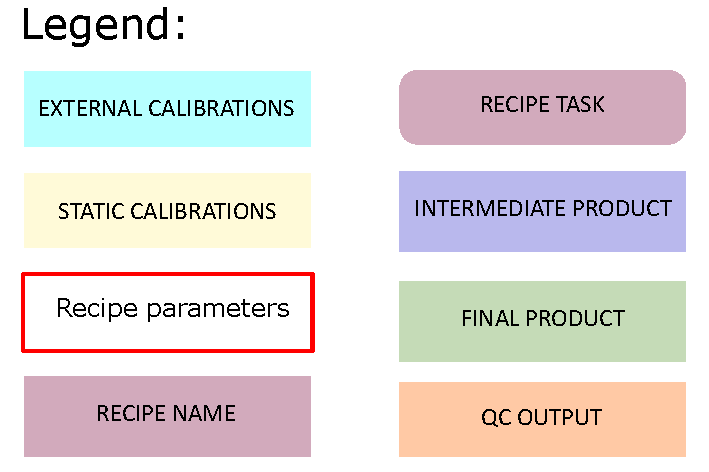
\includegraphics[width=0.4\textheight]{figures/legend.pdf}
  \caption[Legend]{Legend of the coloured boxes in the \ac{LSS} cascades.}
  \label{Fig:LSScascadelegend}
\end{figure}
\clearpage

\begin{sidewaysfigure}[ht]
  \centering
  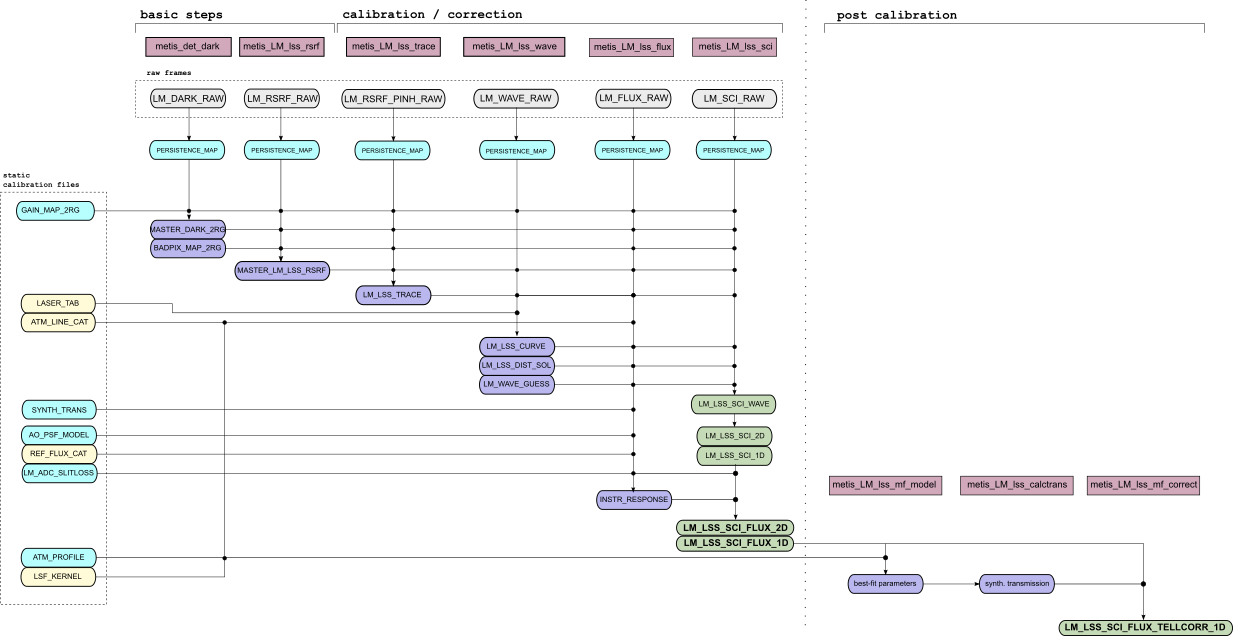
\includegraphics[width=0.9\textheight]{figures/LM_LSS_pipeline_wf_draft_latest_v0.74.png}
  \caption[Reduction cascade and association map for LM long-slit
  spectroscopy]{Reduction cascade and association map for long-slit
    spectroscopy in the LM bands.  }
  \label{Fig:LMLssAssomap}
\end{sidewaysfigure}



% \begin{sidewaysfigure}[ht]
%   \centering
%   \includegraphics[width=0.9\textheight]{figures/NQ_LSS_pipeline_wf_draft_latest.png}
%   \caption[Reduction cascade and association map for N long-slit
%   spectroscopy]{Reduction cascade and association map for long-slit
%     spectroscopy in the N band.  }
%   \label{Fig:NQLssAssomap}
% \end{sidewaysfigure}


%% ---- Table: LM long-slit spectroscopy
\begin{sidewaystable}
  \footnotesize
  \begin{center}
    \caption[Data Processing table for LM long-slit spectroscopy]{%
      Data Processing table for LM long-slit spectroscopy
      calibration mode; }\bigskip
    \label{Tab:LMLssDatProc}
    \begin{tabular}{|l|l|l|l|l|l|}
      \hline
      Data Type   & Classification & Recipe (Level)	& FITS Keywords & static CalibDB & Products\\
    (Templates) & Keywords	 & Processing steps	&		&	  &	\\
    \hline
    \TPL{DARK}	& \CODE{DPR.CATG==CALIB} & \hyperref[sssec:metis_det_dark]{\REC{metis_det_dark}} & Exposure time	&	\hyperref[dataitem:gainmap2rg]{\PROD{GAIN_MAP_2RG}}& Averaged dark frame\\
    		& \CODE{DPR.TYPE==DARK}  &			&		&	& Bad pixel map\\
    		& \CODE{DPR.TECH==IMAGE}  &			&		&	& \\
    \hline
    \TPL{FLAT}	& \CODE{DPR.CATG==CALIB} & \hyperref[rec:lsslmrsrf]{\REC{metis_LM_lss_rsrf}} & Exposure time	& \hyperref[dataitem:gainmap2rg]{\PROD{GAIN_MAP_2RG}}	& Averaged, normalized flatfield\\
    		& \CODE{DPR.TYPE==FLAT}  &			&	Grism	& 	& \\
    		& \CODE{DPR.TECH==SPECTRUM}  &			&	Slit	&	& \\
    \hline
         	& \CODE{DPR.CATG==CALIB} &\hyperref[rec:lsslmtrace]{\REC{metis_LM_lss_trace}} & Exposure time	& \hyperref[dataitem:gainmap2rg]{\PROD{GAIN_MAP_2RG}}	& Order location\\
    		& \CODE{DPR.TYPE==FLAT}  &			&		&	& (polynomial fit)\\
    		& \CODE{DPR.TECH==SPECTRUM}  &			&		&	& \\
    \hline
    \TPL{WAVE,LASER} & \CODE{DPR.CATG==CATG} &\hyperref[rec:lsslmwave]{\REC{metis_LM_lss_wave}} & Exposure time &  \hyperref[dataitem:gainmap2rg]{\PROD{GAIN_MAP_2RG}} & wavelength solution\\
    		& \CODE{DPR.TYPE==WAVE,LASER}   &			   & Grism & \hyperref[dataitem:lasertab]{\STATCALIB{LASER_TAB}} &\\
    		& \CODE{DPR.TECH==SPECTRUM}  &			& Slit		&	& \\
    		& \CODE{PRO.CATG==SPECTRUM}   &  &  & & \\
    \hline
    \TPL{FLUX,STD} & \CODE{DPR.CATG==CALIB} & \hyperref[rec:lsslmflux]{\REC{metis_LM_lss_flux}}& Object name (Flux STD) & \hyperref[dataitem:gainmap2rg]{\PROD{GAIN_MAP_2RG}} & Instrumental\\
    		& \CODE{DPR.TYPE==FLUX,STD}   &			   & Exposure time & \hyperref[dataitem:atmlinecat]{\EXTCALIB{ATM_LINE_CAT}} & response function\\
    		& \CODE{DPR.TECH==SPECTRUM}  &			&	Grism	&	\hyperref[dataitem:lmsynthtrans]{\STATCALIB{LM_SYNTH_TRANS}}& \\
    		& \CODE{PRO.CATG==SPECTRUM}   &  & Slit & \hyperref[dataitem:lmadcslitloss]{\STATCALIB{LM_ADC_SLITLOSS}} & \\
    		& & & & \hyperref[dataitem:aopsfmodel]{\EXTCALIB{AO_PSF_MODEL}} &\\    
    		& & & & \hyperref[dataitem:reffluxcat]{\STATCALIB{REF_FLUX_CAT}} &\\    \hline
    \TPL{SCIENCE} & \CODE{DPR.CATG==SCIENCE} & \hyperref[rec:lsslmsci]{\REC{metis_LM_lss_sci}} & Object name &  \hyperref[dataitem:gainmap2rg]{\PROD{GAIN_MAP_2RG}} & Science grade spectrum\\
    		& \CODE{DPR.TYPE==OBJECT}   &			   & Exposure time & \hyperref[dataitem:lmadcslitloss]{\STATCALIB{LM_ADC_SLITLOSS}} &\\
    		& \CODE{DPR.TECH==SPECTRUM}  &			&	Grism	& \hyperref[dataitem:atmlinecat]{\EXTCALIB{ATM_LINE_CAT}}	& \\
    		& \CODE{PRO.CATG==SPECTRUM}   &  & Slit  &  & \\
    \hline
            & \CODE{DPR.CATG==SCIENCE} & \hyperref[rec:LMLSSmfmodel]{\REC{metis_LM_lss_mf_model}} & Object name & \hyperref[dataitem:lsfkernel]{\STATCALIB{LSF_KERNEL}}	 & Best-fit \\
    		& \CODE{DPR.TYPE==OBJECT}   &			  & & \hyperref[dataitem:atmprofile]{\EXTCALIB{ATM_PROFILE}}  & \texttt{molecfit} parameters\\
    		& \CODE{DPR.TECH==TBD}  &			&		& \hyperref[dataitem:atmlinecat]{\EXTCALIB{ATM_LINE_CAT}}	& \\
    		& \CODE{PRO.CATG==TBD}   &  &  & start parameter set & \\
    \hline
            & \CODE{DPR.CATG==SCIENCE} &  \hyperref[rec:LMLSSmfcalctrans]{\REC{metis_LM_lss_mf_calctrans}} & Object name & \hyperref[dataitem:atmlinecat]{\EXTCALIB{ATM_LINE_CAT}}	 & synthetic \\
    		& \CODE{DPR.TYPE==LSS}   &		&	   &   & Transmission curve\\
    		& \CODE{DPR.TECH==TBD}  &			&		& 	& \\
    		& \CODE{PRO.CATG==TBD}   &  &  & & \\
    \hline
            & \CODE{DPR.CATG==SCIENCE} &  \hyperref[rec:LMLSSmfcorrect]{\REC{metis_LM_lss_mf_correct}} & Object name & 	 & Absorption corrected\\
    		& \CODE{DPR.TYPE==LSS}   &			   & & synthetic Transmission curve  & science spectrum\\
    		& \CODE{DPR.TECH==TBD}  &			&		&	& \\
    		& \CODE{PRO.CATG==TBD}   &  &  & & \\
    \hline
    \end{tabular}
  \end{center}
\end{sidewaystable}

\begin{sidewaysfigure}[ht]
  \centering
  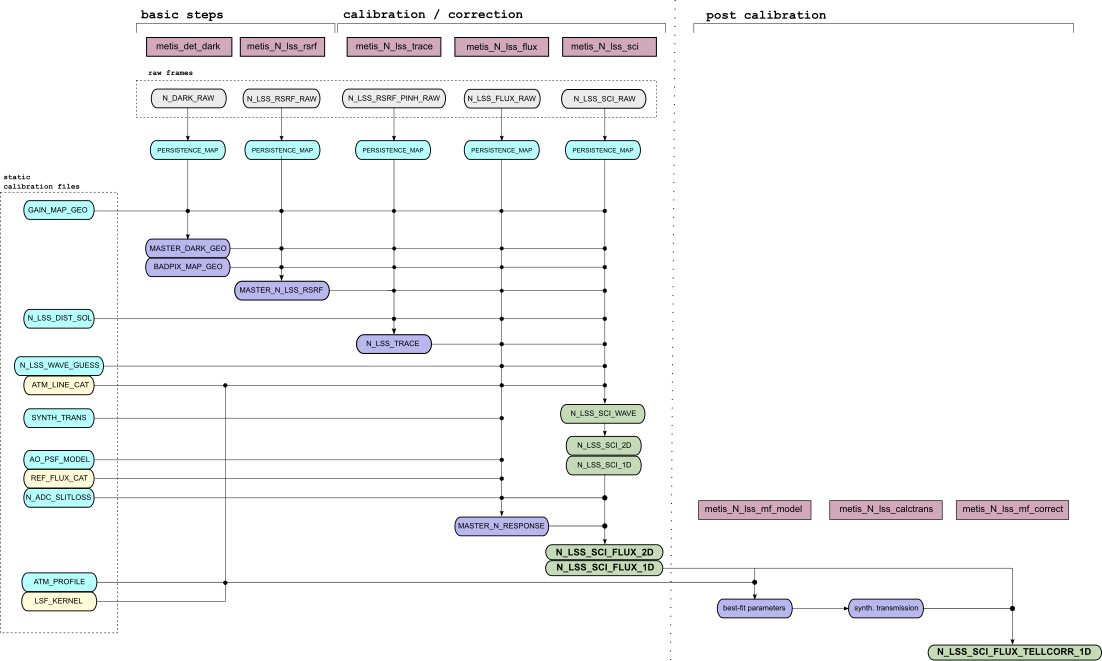
\includegraphics[width=0.9\textheight]{figures/N_LSS_pipeline_wf_draft_latest_v0.74.png}
  \caption[Reduction cascade and association map for N long-slit
  spectroscopy]{Reduction cascade and association map for long-slit
    spectroscopy in the N bands. }
  \label{Fig:NLssAssomap}
\end{sidewaysfigure}

%% ---- Table: N long-slit spectroscopy
\begin{sidewaystable}
  \footnotesize
  \begin{center}
    \caption[Data Processing table for N-band long-slit spectroscopy]{%
      Data Processing table for N long-slit spectroscopy
      calibration mode}\bigskip
    \label{Tab:NLssDatProc}
    \begin{tabular}{|l|l|l|l|l|l|}
      \hline
      Data Type   & Classification & Recipe (Level)	& FITS Keywords & static CalibDB & Products\\
    (Templates) & Keywords	 & Processing steps	&		&	  &	\\
    \hline
    \TPL{DARK}	& \CODE{DPR.CATG==CALIB} & \hyperref[sssec:metis_det_dark]{\REC{metis_det_dark}} & Exposure time	& \hyperref[dataitem:gainmap2rg]{\PROD{GAIN_MAP_GEO}}	& Averaged dark frame\\
    		& \CODE{DPR.TYPE==DARK}  &			&		&	& Bad pixel map\\
    		& \CODE{DPR.TECH==IMAGE}  &			&		&	& \\
    \hline
    \TPL{FLAT}	& \CODE{DPR.CATG==CALIB} & \hyperref[rec:lssnrsrf]{\REC{metis_N_lss_rsrf}} & Exposure time	& \hyperref[dataitem:gainmap2rg]{\PROD{GAIN_MAP_GEO}}	& Averaged, normalized flatfield (\ac{RSRF}\\
    		& \CODE{DPR.TYPE==FLAT}  &			&	Grism	&	& Bad pixel map\\
    		& \CODE{DPR.TECH==SPECTRUM}  &			& Slit		&	& \\
    \hline
         	& \CODE{DPR.CATG==CALIB} & \hyperref[rec:lssntrace]{\REC{metis_N_lss_trace} }& Exposure time	& \hyperref[dataitem:gainmap2rg]{\PROD{GAIN_MAP_GEO}}	& Order location\\
    		& \CODE{DPR.TYPE==FLAT}  &			&	Grism	&	& (polynomial fit)\\
    		& \CODE{DPR.TECH==SPECTRUM}  &			&	Slit	&	& \\
    \hline
    \TPL{FLUX,STD} & \CODE{DPR.CATG==CALIB} & \hyperref[rec:lssnflux]{\REC{metis_N_lss_flux}} & Object name (Flux STD) & \hyperref[dataitem:gainmap2rg]{\PROD{GAIN_MAP_GEO}} & Instrumental\\
    		& \CODE{DPR.TYPE==FLUX,STD}   &			   & Exposure time & \hyperref[dataitem:nlsswaveguess]{\STATCALIB{N_LSS_WAVE_GUESS}} & response function\\
    		& \CODE{DPR.TECH==SPECTRUM}   &			   & Grism		& \hyperref[dataitem:atmlinecat]{\EXTCALIB{ATM_LINE_CAT}}	& \\
    		& \CODE{PRO.CATG==SPECTRUM}   &  &  Slit & \hyperref[dataitem:nsynthtrans]{\STATCALIB{N_SYNTH_TRANS}} & \\
    		& & & & \hyperref[dataitem:nadcslitloss]{\STATCALIB{N_ADC_SLITLOSS}} &\\
    		& & & &  \hyperref[dataitem:reffluxcat]{\STATCALIB{REF_FLUX_CAT}} &\\
    		& & & & \hyperref[dataitem:aopsfmodel]{\EXTCALIB{AO_PSF_MODEL}} &\\
    		& & & & \hyperref[dataitem:nlssdistsol]{\STATCALIB{N_LSS_DIST_SOL}} &\\
    		& & & & \hyperref[dataitem:reffluxcat]{\STATCALIB{REF_FLUX_CAT}} &\\
    \hline
    \TPL{SCIENCE} & \CODE{DPR.CATG==SCIENCE} & \hyperref[rec:lssnsci]{\REC{metis_N_lss_sci}} & Object name & \hyperref[dataitem:gainmap2rg]{\PROD{GAIN_MAP_GEO}}  & Science grade spectrum\\
    		& \CODE{DPR.TYPE==OBJECT}   &			   & Exposure time &  \hyperref[dataitem:atmlinecat]{\EXTCALIB{ATM_LINE_CAT}} &\\
    		& \CODE{DPR.TECH==SPECTRUM}  &			&	Grism	&\hyperref[dataitem:nadcslitloss]{\STATCALIB{N_ADC_SLITLOSS}}	& \\
    		& \CODE{PRO.CATG==SPECTRUM}   &  & Slit & \hyperref[dataitem:nlsswaveguess]{\STATCALIB{N_LSS_WAVE_GUESS}} & \\
    		& & & & \hyperref[dataitem:nlssdistsol]{\STATCALIB{N_LSS_DIST_SOL}} &\\
    \hline
            & \CODE{DPR.CATG==SCIENCE} & \hyperref[rec:NLSSmfmodel]{\REC{metis_N_lss_mf_model}} & Object name & \hyperref[dataitem:lsfkernel]{\STATCALIB{LSF_KERNEL}}	 & Best-fit \\
    		& \CODE{DPR.TYPE==OBJECT}   &			  & & \hyperref[dataitem:atmprofile]{\EXTCALIB{ATM_PROFILE}}  & \texttt{molecfit} parameters\\
    		& \CODE{DPR.TECH==TBD}  &			&		& \hyperref[dataitem:atmlinecat]{\EXTCALIB{ATM_LINE_CAT}}	& \\
    		& \CODE{PRO.CATG==TBD}   &  &  & start parameter set & \\
    \hline
            & \CODE{DPR.CATG==SCIENCE} & \hyperref[rec:NLSSmfcalctrans]{\REC{metis_N_lss_mf_calctrans}} & Object name & \hyperref[dataitem:atmlinecat]{\EXTCALIB{ATM_LINE_CAT}}	 & synthetic \\
    		& \CODE{DPR.TYPE==LSS}   &		&	   &  & Transmission curve\\
    		& \CODE{DPR.TECH==TBD}  &			&		&  	& \\
    		& \CODE{PRO.CATG==TBD}   &  &  & & \\
    \hline
            & \CODE{DPR.CATG==SCIENCE} & \hyperref[rec:NLSSmfcorrect]{\REC{metis_N_lss_mf_correct}} & Object name & 	 & Absorption corrected\\
    		& \CODE{DPR.TYPE==LSS}   &			   &  & synthetic Transmission curve & science spectrum\\
    		& \CODE{DPR.TECH==TBD}  &			&		&	& \\
    		& \CODE{PRO.CATG==TBD}   &  &  & & \\
    \hline
    \end{tabular}
  \end{center}
\end{sidewaystable}

\subsubsection{Static calibration database}\label{lss:static_calib}
The static calibration database comprises several data sets, some are updated from time to time:
\begin{itemize}
    \item \hyperref[dataitem:gainmap2rg]{\hyperref[dataitem:gainmap2rg]{\PROD{GAIN_MAP_2RG}}} and \hyperref[dataitem:gainmapgeo]{\hyperref[dataitem:gainmap2rg]{\PROD{GAIN_MAP_GEO}}}: These are the detector gain maps of the detectors (2RG=Hawaii2RG, LM-band; GEO=Geosnap, N-band), which are created by the recipe \hyperref[sssec:metis_det_lingain]{\REC{metis_det_lingain}} (see Section~\ref{sssec:metis_det_lingain}). This recipe also checks the linearity of the pixels and is carried out every once in a while (yearly, TBD, see \cite{METIS-calibration_plan}) as we assume the detectors to be fairly stable.
    \item \hyperref[dataitem:lasertab]{\STATCALIB{LASER_TAB}}: The \ac{WCU} provides laser sources for the first guess of the wavelength solution. The main laser frequencies are fixed (\cite{METIS-calibration_plan}) and given in a static table.
    \item \hyperref[dataitem:atmlinecat]{\EXTCALIB{ATM_LINE_CAT}}: The main wavelength calibration will be done by means of atmospheric lines, most probably based on the \ac{HITRAN}\footnote{\url{https://hitran.org/}}. They are given in a static catalogue. This database is also required by the telluric correction package \texttt{molecfit}.
    \item \hyperref[dataitem:lmsynthtrans]{\STATCALIB{LM_SYNTH_TRANS}}/\hyperref[dataitem:nsynthtrans]{\STATCALIB{N_SYNTH_TRANS}}: For the determination of the continuum of flux standard stars a rough telluric correction is needed. We intend to apply static transmission curves for that purpose as we deem it to be sufficient and more time efficient than applying the telluric correction package \texttt{molecfit} every time. This static transmission curve will be determined during commissioning via \texttt{molecfit}.
    \item \hyperref[dataitem:aopsfmodel]{\EXTCALIB{AO_PSF_MODEL}}: For the determination of \ac{AO}-induced slit losses we intend to use a static \ac{PSF} model, which is scaled by the \ac{AO} telemetry data. Details on that are TBD.
    \item \hyperref[dataitem:reffluxcat]{\STATCALIB{REF_FLUX_CAT}}: The absolute flux calibration will be done by observations of specific flux standard stars, which are compared to their theoretical models. The \hyperref[dataitem:reffluxcat]{\STATCALIB{REF_FLUX_CAT}} will contain these models. Currently, the catalogue of flux standard stars comprises the stars from the catalogue of the \ac{VISIR} instrument.
    \item \hyperref[dataitem:lmadcslitloss]{\STATCALIB{LM_ADC_SLITLOSS}}/\hyperref[dataitem:nadcslitloss]{\STATCALIB{N_ADC_SLITLOSS}}: It is expected that the fixed positions of the \ac{ADC} will introduce specific slit losses. These losses are determined in the recipes \hyperref[rec:metislmadcmslitloss]{\REC{metis_lm_adc_slitloss}} and \hyperref[rec:metisnadcmslitloss]{\REC{metis_n_adc_slitloss}} (see Section~\ref{sssec:adc_slitlosses} and \cite{METIS-calibration_plan}). As these losses are assumed to be very stable, these recipes will be carried out only rarely.
    \item \hyperref[dataitem:atmprofile]{\EXTCALIB{ATM_PROFILE}} and \hyperref[dataitem:lsfkernel]{\STATCALIB{LSF_KERNEL}}: The telluric correction package \texttt{molecfit} requires an atmospheric profile incorporating height information of the temperature, pressure and molecular abundances as input. Currently we use a static profile (equatorial \texttt{equ.atm}\footnote{\url{https://eodg.atm.ox.ac.uk/RFM/atm/}}) as starting point of the fit of the molecular column densities. In addition, a kernel for the \ac{LSF} is provided. We intend to determine the kernel during commissioning and use this as input. However, it is still unclear in how far the \ac{AO} influences that kernel. The current baseline is to use the static \hyperref[dataitem:lsfkernel]{\STATCALIB{LSF_KERNEL}} as starting point for fitting the line spread function.
    \item \hyperref[dataitem:nlssdistsol]{\STATCALIB{N_LSS_DIST_SOL}}/\hyperref[dataitem:nlsswaveguess]{\STATCALIB{N_LSS_WAVE_GUESS}}: First guess solutions of the N-band LSS mode are static due to the absence of laser sources after \ac{AIT}. As the instrument is expected to be very stable, these calibration files will be created only once and kept static.
\end{itemize}